\section[Semiconductor Devices]{\hyperlink{toc}{Semiconductor Devices}}



\textbf{Heterostructures}: Layers of 2 or more different semiC - band strucutre design.


Lattice mismaatch negligile -- heterojunction = single crystal with different site occupancies across juntion.


3 types of band edge offsets:
\begin{enumerate}
    \item Normal
    \item Staggered
    \item Broken Gap
\end{enumerate}

\begin{itemize}
    \item To make a clean growth of heterostructures you want to match lattice constants (a) very closely
    \item if it is not matched you will get strain in your sample, and you will get deffects in your grown sample.
    
    \item \textbf{Transmission Electron Microscope (TEM):} send electrons at very high energy all the way through the structure, and pixels represent atomic rows. tells you about the crystallinity of the structure under study.
    
    \item \textbf{Molecular Beam Epitaxy (MBE)}: The structures are gorwn in MBE machines. It generates beams of molecules, and grow layer by layer (epitaxially). 
    \item Stainless steal \textbf{ultra high vacuum chamber} so that beams of molecules can go in straight lines and not collide with anything (massive mean free path).
    \item \textbf{Diffusion cells} (molecular guns): buckets containing different materials, heated to a certain temperature where material begins to sublimate.
    \item \textbf{Substrate} is the base on which you grown an epitaxial thin film.
    \item Overlap of for ex. Ga and As shooting at the same time onto the substrate allows for growth of GaAs.
    \item \textbf{ Reflection High Energy Electron Diffraction (RHEED):} Shoots electrons at sample which reflect and hit screen while the sample is being grown. Intensity of diffraction pattern oscillates as you're growing. Used to count the layers grown so far.
    \item RHEED: max diffraction pattern intensity at new layer, min at half layer, max at completion of a layer. layer by layer we can see and count the layers that have been grown so far.
    \item \textbf{Quantum Wells:} \begin{equation}
        E = n^2 \frac{\hbar^2 \pi^2}{2m_eL_z^2} \qquad \in n =1,2,3.
    \end{equation} 
    \item \textbf{Gas LASER:} for ex HeNe works on the atomic transitions within the gas, and uses some kind of pump to bring all the atoms into the excited state and they relax and emit photons all with the same energy. usese mirror structure to boost this process.
    \item \textbf{Quantum Well Laser (27:00):} pumping by sending electrical current through. 
    \item \textbf{Quantum Cascade Laser:} electrons falls from one QW to the next each time emitting a photon of a specific energy.
    \item \textbf{Field Effect Transistor (HEMT- High electron mobility transistor):} 3 components - source, gate and drain
    \item \textbf{2DEG: Two Dimensional Electron Gas}
    \item \textbf{PN Junction (Diode):} When N-type and P-type dopants are introduced side-by-side in a semiconductor, a PN junction or diode is formed. \item \textbf{Rectifier Circuits:} converts an AC voltage into a DC voltage.Sin wave negative values are cut off by diodes unidirectional feature. 
    \item \textbf{Light Emitting Diodes (LED):} Recombination in the middle of the PN junction diode of the electron and hole emits a photon. Band gap of the junction determines the colour of the photon.
    \item Blue LEDs won a nobel prize recently with nitride based diodes.
    \item \textbf{Bandgap Engineering:}
    \begin{figure}
    \centering
    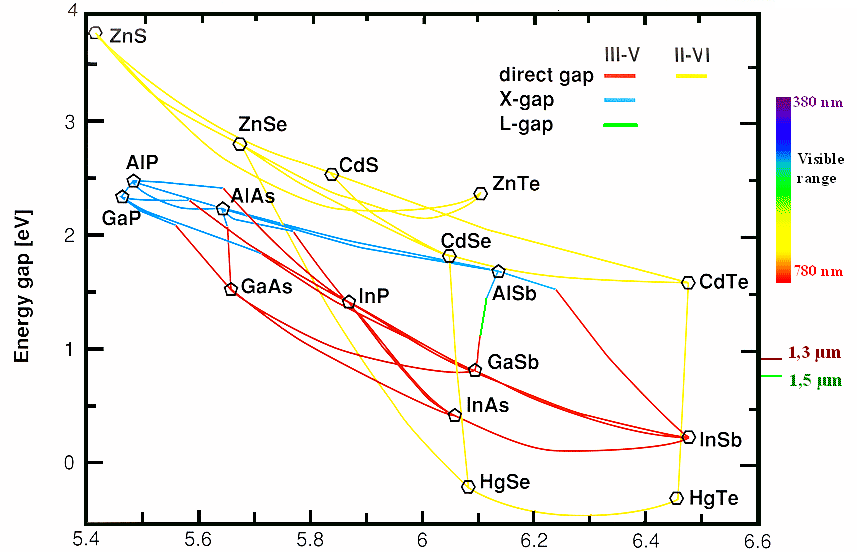
\includegraphics[width=0.75\linewidth]{Images/bandgap_misfit.png}
    \caption{bandgap}
    \label{fig:bandgapengineering}
    \end{figure}
    Tweaking structures to tune the wavelength and the properties.
    \item \textbf{Solar Cells:} Photon comes in and excites an electron-hole pair in a PN junction. The charges separate and this produces a current.
    \item \textbf{Schottky Barrier:} Metal-SemiC Junction.
    \item \textbf{Metal-Oxide-Semiconductor Transistors:} Most modern digital devices use MOS transistors. Greater density and simpler geometry (easier to make). Switch on and off more slowly. 
    \item Consists of source, drain diffusions, with a gate that controls whether the transistor. 
    \item MOSFET: Metal-Oxide Semiconductor Field Effect Transistor.
    \item Applying positive gate voltage (attracts electrons to gate area, i.e. a conductive path),causes current to flow from source to drain. The more voltage, the more current.  
    \item negative current in MOSFET is like two diodes facing each other (both directions blocked).
    \item \textbf{Complementary MOS Transistors:} Use transistors for logic circuits.
    \item \textbf{Integrated Circuit (IC) chips:} 12 inch semiC wafer printed at INTEL with nanofabrication. out of silicon with n and p doped regions and metal contacts. chopped up into chips to be put into our laptops. They are filled with hundreds of millions of MOSFETS.
    \item \textbf{Electric Field in a CCD:} Charge coupled device. Pixel in our digital camera. Also functions with a P-N junction.

\end{itemize}